\documentclass{article}

\usepackage[T2A]{fontenc}
\usepackage[utf8]{inputenc}
\usepackage[english, russian]{babel}

\usepackage{amssymb, amsmath, eucal, latexsym, amsthm}
\usepackage{epstopdf}
\usepackage{graphicx}

\newtheorem*{theorem}{Теорема}
\newtheorem*{definition}{Определение}

\begin{document}

\title{Теорема о линейном операторе}

\maketitle

Рассматривается дифференциальное уравнение второго порядка с периодичной правой частью:
\begin{equation}
	u_{xx} = f(x, u), \quad f(x + L, u) = f(x, u).
\label{eq:initial}
\end{equation}
Функция $f(x, u)$ достаточно хорошая.
Периодичность правой части позволяется ввести отображение Пуанкаре $\mathcal{P}: \mathbb{R}^2 \to \mathbb{R}^2$ за период $L$, связанное с этим уравнением.
\begin{equation}
	\mathcal{P} \begin{pmatrix} u_0 \\ u_0' \end{pmatrix}
	= \begin{pmatrix} u_L \\ u_L' \end{pmatrix},
\end{equation}
где $u_L = u(L)$, $u_L' = u'(L)$, а $u(x)$ является решением уравнения \eqref{eq:initial} с начальными условиями $u(0) = u_0$, $u'(0) = u_0'$.
Отображение Пуанкаре может быть определено не на всей фазовой плоскости $\mathbb{R}^2$, а лишь на некотором её подмножестве.
Для дальнейшего изложения важно, чтобы область определения отображения $\mathcal{P}$ представляла из себя так называемое {\it островное множество}.

\begin{definition}
	Назовём {\bf островом} криволинейный четырехугольник $D \subset \mathbb{R}^2$ на фазовой плоскости $(u, u')$, образованный двумя парами непересекающихся кривых $\alpha^{\pm}$, $\beta^{\pm}$, при этом:
	\begin{itemize}
		\item кривые $\alpha^{\pm}$ являются графиками монотонных $\gamma$-липшицевых функций $u' = h_{\pm}(u)$;
		\item кривые $\beta^{\pm}$ являются графиками монотонных $\gamma$-липшицевых функций $u = v_{\pm}(u')$;
		\item если функции $h_{\pm}(u)$ являются возрастающими, тогда функции $v_{\pm}(u')$ -- убывающие, и наоборот, если функции $h_{\pm}(u)$ являются убывающими, тогда $v_{\pm}(u')$ -- возрастающие.
	\end{itemize}
\end{definition}

\begin{definition}
	Назовём множество $\mathcal{D} = \bigcup_{i = 0}^{\infty} D_i$ {\bf островным}, если оно представляет из себя счётное объединение взаимно непересекающихся островов.
\end{definition}

\begin{figure}[h]
\centering
  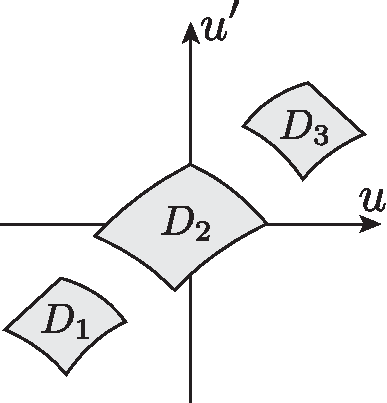
\includegraphics[scale = 0.8]{pic/set of islands}
  \caption{Пример островного множества $\mathcal{D}$ из 3-х островов.}
\label{fig:islands}
\end{figure}

Далее на островном множестве $\mathcal{D}$ введем определения $v$, $h$~-~кривых и $v$, $h$~-~полос соответственно.

\begin{definition}
	Пусть $D \in \mathcal{D}$ -- остров, ограниченный кривыми $\alpha^{\pm}$, $\beta^{\pm}$.
	Рассмотрим кривую $\beta$, соединяющую противолежащие стороны $\alpha^{\pm}$ острова $D$.
	Назовём такую кривую $\mathbf{v}$-{\bf кривой}, если она является графиком монотонной $\gamma$-липшицевой функции $u = v(u')$, при этом тип монотонности этой функции совпадает с типом монотонности функций $u = v_{\pm}(u')$ соответствующих границам $\beta^{\pm}$ острова $D$.
\end{definition}

\begin{definition}
	Аналогично назовём кривую $\alpha$, соединяющую границы $\beta^{\pm}$, $\mathbf{h}$-{\bf кривой}, если она является графиком монотонной $\gamma$-липшицевой функции $u' = h(u)$, при этом тип её монотонности совпадает с типом монотонности границ $\alpha^{\pm}$ острова $D$.
\end{definition}

Введенные определения проиллюстрированы на рисунках \ref{fig:islands} и  \ref{fig:curves-and-strips}.

\begin{figure}[h]
\centering
  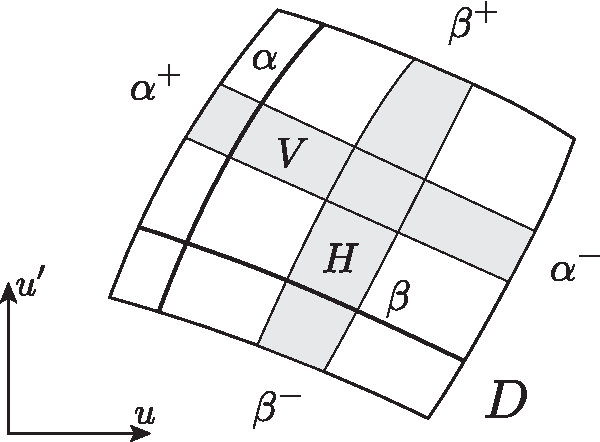
\includegraphics[scale = 0.8]{pic/curves and strips}
  \caption{Остров $D$ с границами $\alpha^+$, $\alpha^-$, $\beta^+$, $\beta^-$; h-кривая $\alpha$, v-кривая $\beta$, h-полоса $H$, v-полоса $V$.}
\label{fig:curves-and-strips}
\end{figure}

\begin{theorem}[{\bf О линейном операторе}]

\end{theorem}

\begin{proof}
	
\end{proof}

\section*{Приложения}

\paragraph{Случай общего положения.} 

Можно просканировать фазовую плоскость с некоторым шагом и просчитать матрицы линейного оператора на множествах $T D_i \cap D_j$ и $T^{-1} D_i \cap D_j$, $\forall i, j$.

\paragraph{Асимптотический предел.}

Области определения внутри островов оказываются вмонтированы в асимптотические разложения.
Можно исследовать матрицы линейного оператора в асимптотическом пределе для каждой пары островов $D_i$, $D_j$.

\end{document}
